\subsection{Refinement of graph rewriting rules}

\begin{definition}[Refinement of two rewriting rules using positive influence]
  \label{def:ref_pos_infl}
  Let $r_1:L_1\remb K_1 \lemb R_1$ and $r_2:L_2\remb K_2 \lemb R_2$ be two rules and let $s$ be a cospan such that $r_1\redl{+}_s r_2$. Define the refinement of $r_1$ and $r_2$ using $s$, $r_1\oplus_s r_2 = M_1\remb K\lemb M_2$ obtained as follows:
  \begin{itemize}
  \item $R_1\lemb M\remb L_2$ is the pushout of the cospan $R_1\remb O \lemb L_2$;
  \item $M_1\Rightarrow M$ is obtained by a dpo rewriting of $M$ using $r_1^{-1}$;
  \item $M\Rightarrow M_2$ is obtained by a dpo rewriting of $M$ using $r_2$;
  \item $D_1\remb K\lemb D_2$ is the pullback of the span $D_1\lemb M \remb D_2$.
  \end{itemize}
  \[
  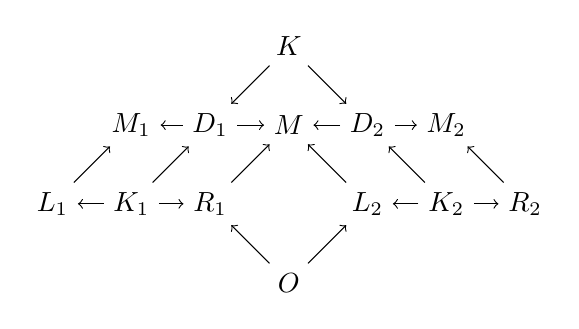
\begin{tikzpicture} %[scale=0.8]
  \node (o) at (0,-1) {\(O\)};
  \node (m) at (0,1) {\(M\)};
  \node (d2) at (1,1) {\(D_2\)};
  \node (m2) at (2,1) {\(M_2\)};
  \node (d1) at (-1,1) {\(D_1\)};
  \node (m1) at (-2,1) {\(M_1\)};
  \node (r1) at (-1,0) {\(R_1\)};
  \node (k1) at (-2,0) {\(K_1\)};
  \node (l1) at (-3,0) {\(L_1\)};
  \node (l2) at (1,0) {\(L_2\)};
  \node (k2) at (2,0) {\(K_2\)};
  \node (r2) at (3,0) {\(R_2\)};
  \node (k) at (0,2) {\(K\)};
  \draw [->] (o) -- (r1);
  \draw [->] (o) -- (l2);
  \draw [->] (r1) -- (m);
  \draw [->] (k1) -- (r1);
  \draw [->] (k1) -- (l1);
  \draw [->] (k1) -- (d1);
  \draw [->] (l1) -- (m1);
  \draw [->] (l2) -- (m);
  \draw [->] (k2) -- (r2);
  \draw [->] (k2) -- (l2);
  \draw [->] (k2) -- (d2);
  \draw [->] (r2) -- (m2);
  \draw [->] (d1) -- (m);
  \draw [->] (d1) -- (m1);
  \draw [->] (d2) -- (m);
  \draw [->] (d2) -- (m2);
  \draw [->] (k) -- (d1);
  \draw [->] (k) -- (d2);
\end{tikzpicture}
\]
\end{definition}

\autoref{def:ref_pos_infl} ressembles the definition of $E$-concurrent productions~\cite{AlgebraicGR}. However, $E$-concurrent productions combines two sequential dependent transitions into a single one, whereas~\autoref{def:ref_pos_infl} combines rules, linked by positive influence.

\begin{definition}[Refinement of two rewriting rules using positive and negative influence]
  \label{def:ref_pos_neg_infl}
  Let $r_1:L_1\remb K_1 \lemb R_1$ and $r_2:L_2\remb K_2 \lemb R_2$ be two rules.
  \begin{itemize}
  \item Let $s_1:R_1 \overset{o_1}{\lemb} O_1\overset{o_1'}{\remb} L_2$ and $s_2:R_1 \overset{o_2}{\lemb} O_2\overset{o_2'}{\remb} L_2$ be two cospans.
    \[
    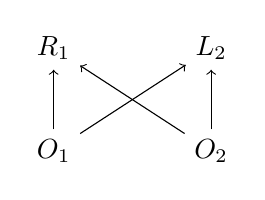
\begin{tikzpicture} %[scale=0.8]
      \node (o) at (1,-1.3) {\(O_2\)};
      \node (o2) at (-1,-1.3) {\(O_1\)};
      \node (r1) at (-1,0) {\(R_1\)};
      \node (l2) at (1,0) {\(L_2\)};
      \draw [->] (o) -- (r1);
      \draw [->] (o) -- (l2);
      \draw [->] (o2) -- (l2);
      \draw [->] (o2) -- (r1);
    \end{tikzpicture}
  \]
  Define $s_1\otimes s_2 = R_1\overset{o_3}{\lemb} O_3\overset{o_3'}{\remb} L_2$ as the cospan constructed as follows:
  \begin{itemize}
  \item let $O_3 = o_1(O_1)\cup o_2(O_2)$ be a subgraph of $R_1$ with $o_3:O_3\subseteq R_1$ the inclusion morphism;
  \item morphism $o_3':O_3\to L_2$ is defined as the union of the morphism $o_1^{-1}\circ o_2:o_1(O_1) \to L_2$ and $o_1'^{-1}\circ o_2':o_2(O_2) \to L_2$, where the morphisms $o_3$ and $o_3'$ are injective, and thus bijective on $\text{image}(O_1)$ and $\text{image}(O_2)$, respectively.
  \end{itemize}
  \item Let $s_1:R_1 \overset{o_1}{\lemb} O_1\overset{o_1'}{\remb} L_2$ be a span such that $r_1\redl{+}_{s_1} r_2$ and let $s_2:L_1 \overset{o_2}{\lemb} O_2\overset{o_2'}{\remb} L_2$ be a cospan such that $r_1\redl{-}_{s_2} r_2$ and $\neg(r_1\redl{-}_{O_2} r_2)$.
    Define $r_1\otimes_{s_1\otimes s_2} r_2 = r_1 \oplus_{s_3} r_2$, obtained as follows:
    \begin{itemize}
    \item if $l_1:K_1\emb L_1$ then $l_1^{-1}:\text{image}(l_1)\emb K_1$;
    \item the morphism $o_2:O_2\emb K_1$ is obtained by the composition of $f:O_2\emb L_1$ and $l_1^{-1}$. Moreover $f(O_2)\subseteq\text{image}(l_1)$ as otherwise, $r_1\redl{-}_{O_2} r_2$, which contradicts the hypothesis;
    \end{itemize}
  \[
  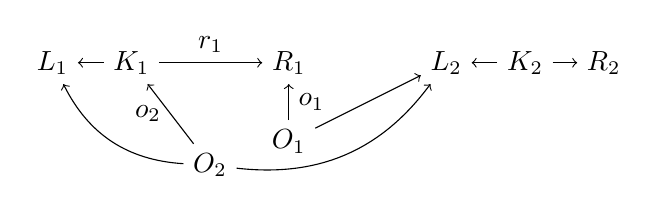
\begin{tikzpicture} %[scale=0.8]
  \node (o) at (-1,-1) {\(O_1\)};
  \node (o2) at (-2,-1.3) {\(O_2\)};
  \node (r1) at (-1,0) {\(R_1\)};
  \node (k1) at (-3,0) {\(K_1\)};
  \node (l1) at (-4,0) {\(L_1\)};
  \node (l2) at (1,0) {\(L_2\)};
  \node (k2) at (2,0) {\(K_2\)};
  \node (r2) at (3,0) {\(R_2\)};
  \draw [->] (o) -- node [right,midway] {\(o_1\)} (r1);
  \draw [->] (o) -- (l2);
  \draw [->] (k1) -- node [above,midway] {\(r_1\)} (r1);
  \draw [->] (k1) -- (l1);
  \draw [->] (k2) -- (r2);
  \draw [->] (k2) -- (l2);
  \draw [->] (o2) to [bend left] (l1);
  \draw [->] (o2) to [bend right] (l2);
  \draw [->] (o2) -- node [left,midway] {\(o_2\)} (k1);
  \end{tikzpicture}
  \]
  \end{itemize}
  %We write $e_1\otimes e_2 = \labl(e_1)\otimes_{O_1,O_2} \labl(e_2)$ to simplify notations.
\end{definition}
